\documentclass{article}

\usepackage{graphicx}
\usepackage{placeins}
\usepackage[subfigure]{ccaption}

\pagestyle{headings}

% italic captions with bold 'figure x'/'table y' texts
\captiontitlefont{\itshape}
\captionnamefont{\bf}


% *** START OF DOCUMENT ***
\begin{document}

\thispagestyle{empty} %no page numbering
\vspace*{4cm}
\centerline{\LARGE \textsc{UDP/IP with VHDL}}
\centerline{\rule{10cm}{1mm}}
\vspace{8cm}
\begin{flushright}
Written by: Jussi Nieminen\\
22.10.2009\\
Tampere University of Technology
\end{flushright}

\newpage

\thispagestyle{empty}
\tableofcontents

\newpage


\pagenumbering{arabic}

\section{INTRODUCTION}
%blaablaablaa, jotain yleista

UDP/IP block is a network interface that is capable of sending and
receiving UDP (User Datagram Protocol) packets over ethernet.  The
block also includes ARP (Address Resolution Protocol) funtionality.
All the source codes are written in VHDL (Very high speed integrated
circuit Hardware Description Language) and licensed under LGPL (Lesser
General Public License).


\subsection{Intended use and restrictions} \label{sec:restrictions}
% mihin on tehty, mita voi tehda, mita ei

This block is originally designed for a Network-on-Chip monitor
application to get high data bandwidth from Altera's DE2 board to a
single PC. (At least higher than with UART.) Future applications in
mind possibility to receive UDP packets sent from a PC was also
included.  This means that the block is desinged for predetermined
communication between two agents using UDP packets only. IP level
broadcasting or network masking are not supported. Correct
functionality when connecting this block to a network full of agents
and protocols is not guaranteed. In addition the size of the used ARP
table (two entries) is not suitable for use in larger networks and
there's no timeouts in cases like ARP request being never answered.

So to wrap things up, without modification this block can be used in
special communication within two agents or in small special networks
using proper UDP packets only. Other types of packets are always
simply discarded. If you need something more advanced, this block
is a good starting point for further development.


\subsection{ARP block} \label{sec:ARP}
% kiitokset ausseille, tehdyt muutokset ja yleiskuvaus
% mainitse rajoituksena arppitaulukon koko

As mentioned, the UDP/IP block also includes ARP functionality. The
internet is a wonderful place, and with little searching ready-made
ARP blocks by Ashley Partis and Jorgen Peddersen~\cite{arp} came up.  The
files were modified to meet our needs (and match our coding style),
but the basic functionality is the same.


\newpage

\section{USAGE}

\subsection{Application side}

This section describes how the UDP/IP block is connected to and
used with an application.

\subsubsection{Interface}

Figure~\ref{fig:appinterface} shows the interface with an application.
Thicker arrows are wider busses while thinner ones stand for single
bit signals. Most of the signals are hopefully self-explanatory. The
rx\_erroneous signal means that the ethernet controller has detected a
possibly data corrupting situation (e.g. collision), but the frame was
nevertheless received. So it's relayed to the application, which can
decide what to do with it.


\begin{figure}[hbt]
  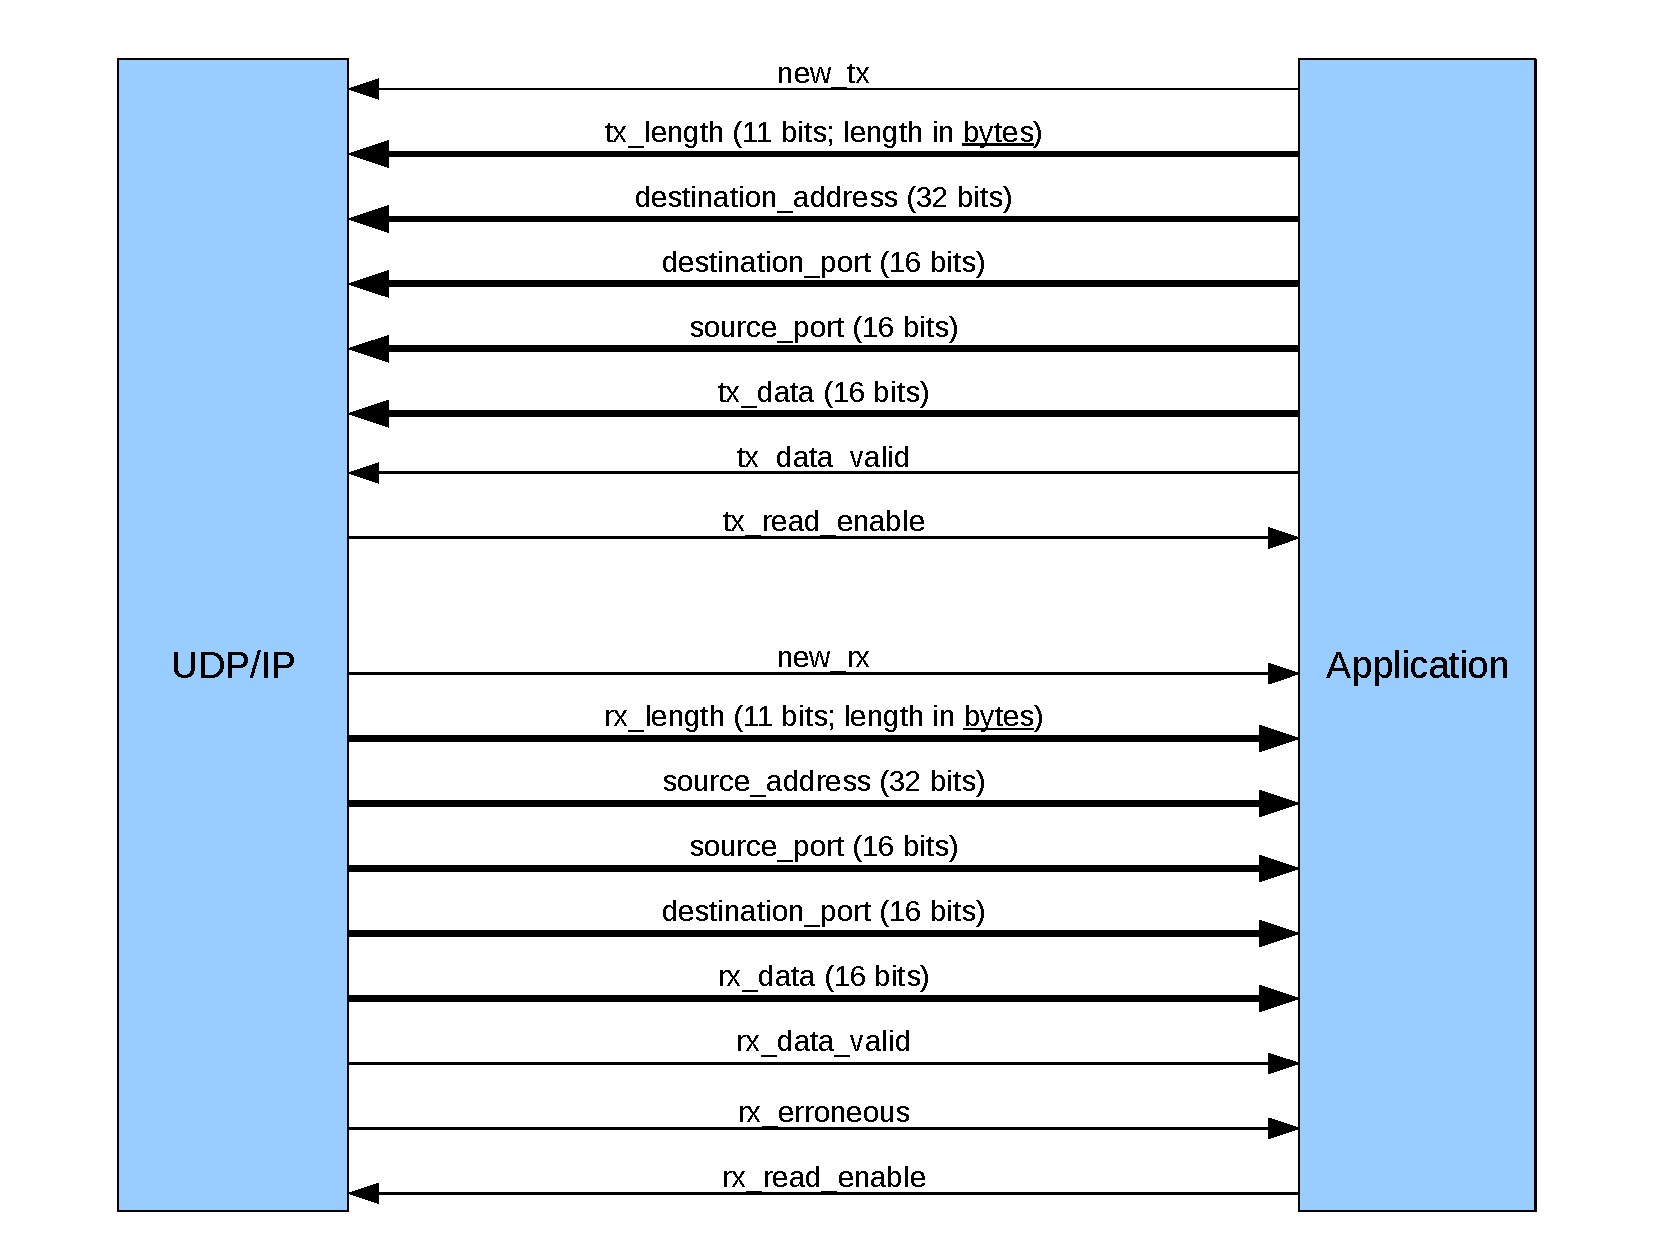
\includegraphics[scale=.5]{fig/app_interface.pdf}
  \caption{Interface between an application and the UDP/IP block.}
  \label{fig:appinterface}
\end{figure}

\subsubsection{About the length and data busses}

As shown in the interface, the length bus is 11 bits wide.  This
corresponds with the maximum possible ethernet frame size (1518
bytes). IP packets could be much longer, but there is no support for
packet fragmenting and thus the maximum possible data length is
maximum ethernet frame size minus headers and ethernet checksum. The
application is responsible for keeping the packet size below maximum.

\begin{displaymath}
  \begin{array}{ll}
    l_{data} & \leq l_{max} - l_{eth} - l_{ip} - l_{udp} - l_{CRC} \\
    & = 1518 - 14 - 20 - 8 - 4 \\
    & = 1472 \textrm{ bytes}
  \end{array}
\end{displaymath}

Length information is given before any data so the application must
know beforehand how much it's going to send. This is due to the fact
that we want to use ethernet controller chip's internal data buffers
to save FPGA resources, and for that (at least some if not all)
ethernet chips need the length beforehand. The application must make
sure, that it really sends or receives data as much as the length
value tells.  \textbf{Remember that the length is given in bytes even
  though data is written two bytes at the time!}

The 16-bit data bus consists of two bytes instead of a single 16-bit
data word. Endianess of the data bus is different from an ethernet
frame (\textit{n~downto~0} versus \textit{0~to~n}), so if you want to
have a sequence 0xABCD on a data frame, you will have to write it as
0xCDAB to the data bus.  If there is a transfer with odd length, the
last byte will use the bits 0 to 7 while bits 8 to 15 can have random
values.  The figure~\ref{fig:dataexample} desperately tries to explain
all this.

\begin{figure}[hbt]
  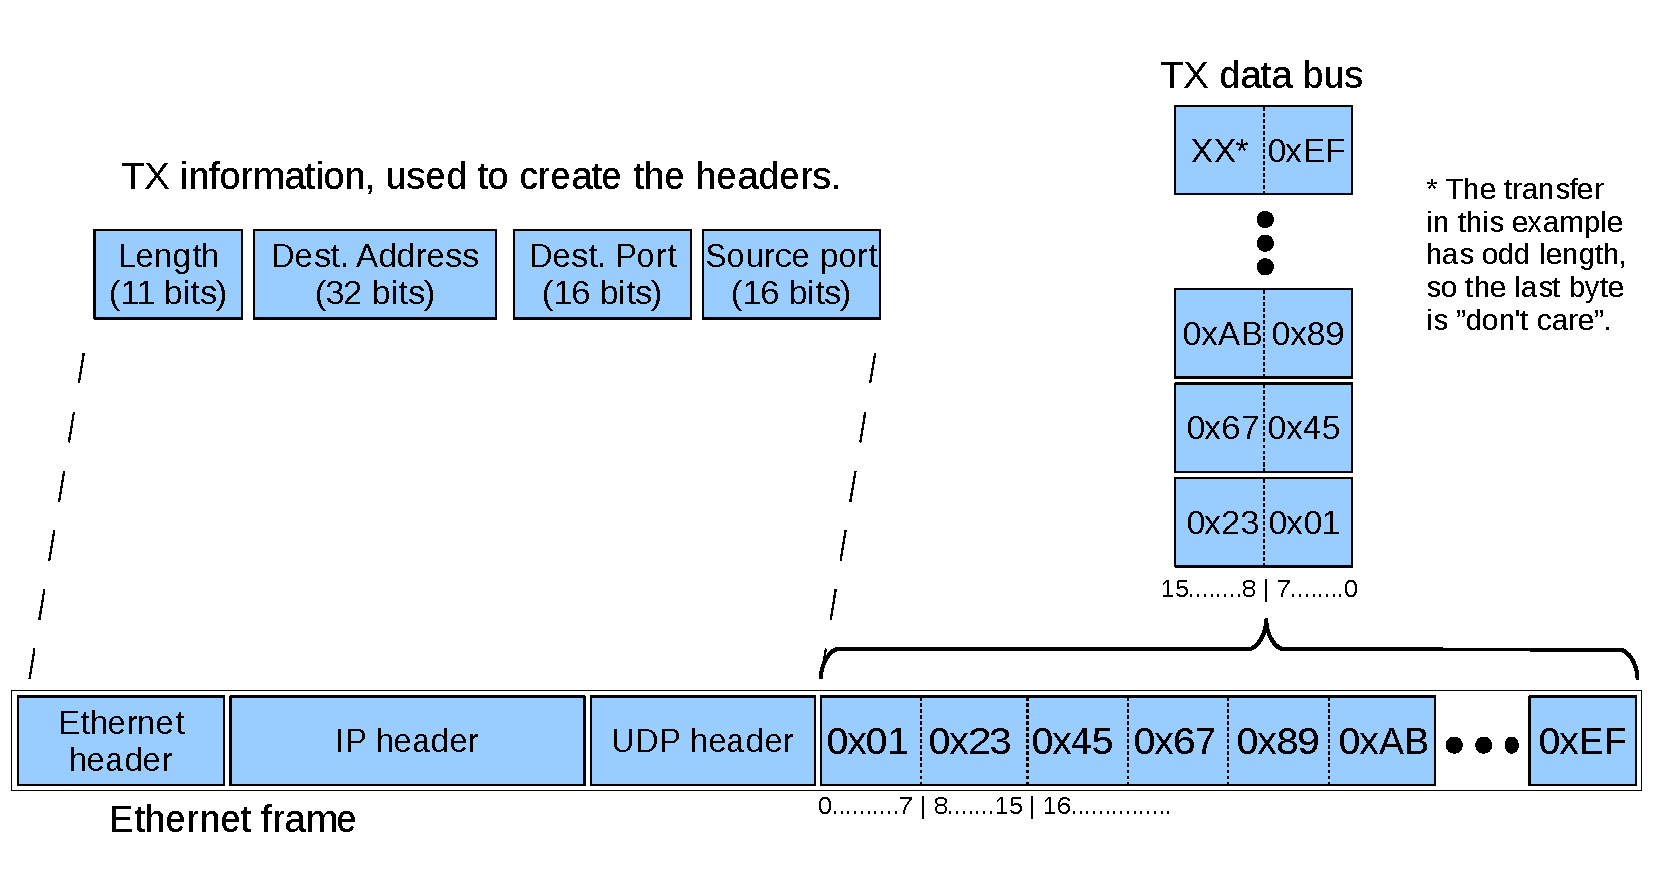
\includegraphics[scale=.5]{fig/data_example.pdf}
  \caption{Example of how the ethernet frame is formed.}
  \label{fig:dataexample}
\end{figure}


\subsubsection{How to get bits running}

Timing for transferring and receiving data is shown in
figure~\ref{fig:timing}.  A new transfer is started by setting up the
new\_tx signal, all the needed information (TX length, destination
address and ports) and the first two bytes of data with data\_valid
signal. When UDP/IP block is ready, it will start reading data by
raising the tx\_read\_enable signal. All the application's signals
must remain stable from the moment new\_tx is risen to the first time
the read enable is up. It might take a while before the UDP/IP block
starts to read if the destination MAC address is not yet in the ARP
table. The first time the read enable is up means that all the other
information (address, ports etc.) has been received and those signals
no longer have to remain the same.

Receiving works exactly the same way, the UDP/IP block sets all the
needed information, first bytes of data and new\_rx signal and
application starts to read by raising up the rx\_read\_enable signal.
The information signals are allowed to change (thus are considered
invalid) once the read enable signal is risen for the first time.

\begin{figure}[hbt]
  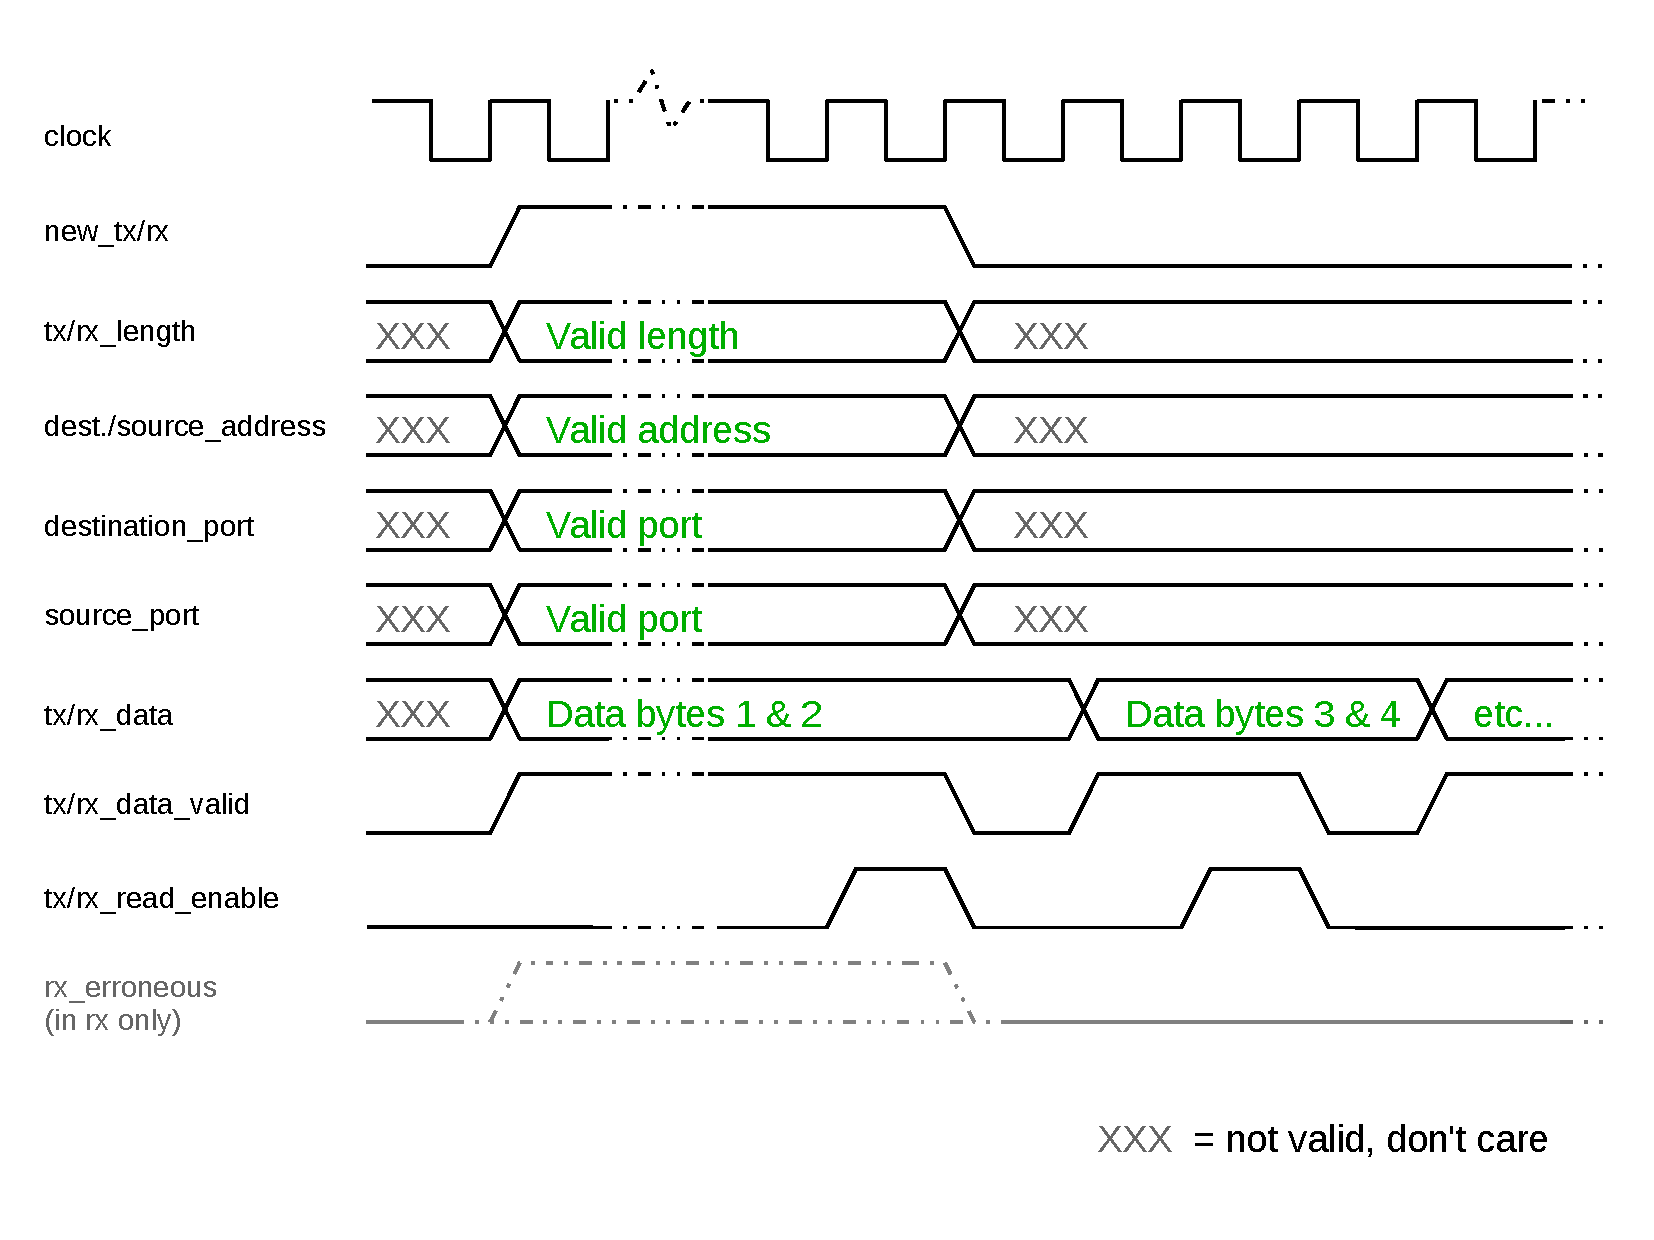
\includegraphics[scale=.5]{fig/tx_timing.pdf}
  \caption{Timing of transferring or receiving data.}
  \label{fig:timing}
\end{figure}


\subsection{Ethernet side}

UDP/IP block's communication with an ethernet controller block is
similar as with an application. Information signals are a bit
different but timing follows the same principle. In fact, when headers
have been written and it's time to write the data the UDP/IP block
simply connects its input and output data signals so that the
application is really talking straight to the ethernet controller
block. More information about this can be found from
section~\ref{sec:implementation}.

\subsubsection{Interface and timing}

Figures \ref{fig:ethinterface} and \ref{fig:ethtiming} contain the
interface and timing information. The ethernet frame type value is
part of an ethernet header and it identifies the protocol that is
carried in that frame. UDP/IP block only accepts frames with frame
types 0x0800 or 0x0806 standing for IP or ARP frames respectively.
Frames with other types are read from the ethernet controller block
but discarded without notifying the application.

\begin{figure}[hbt]
  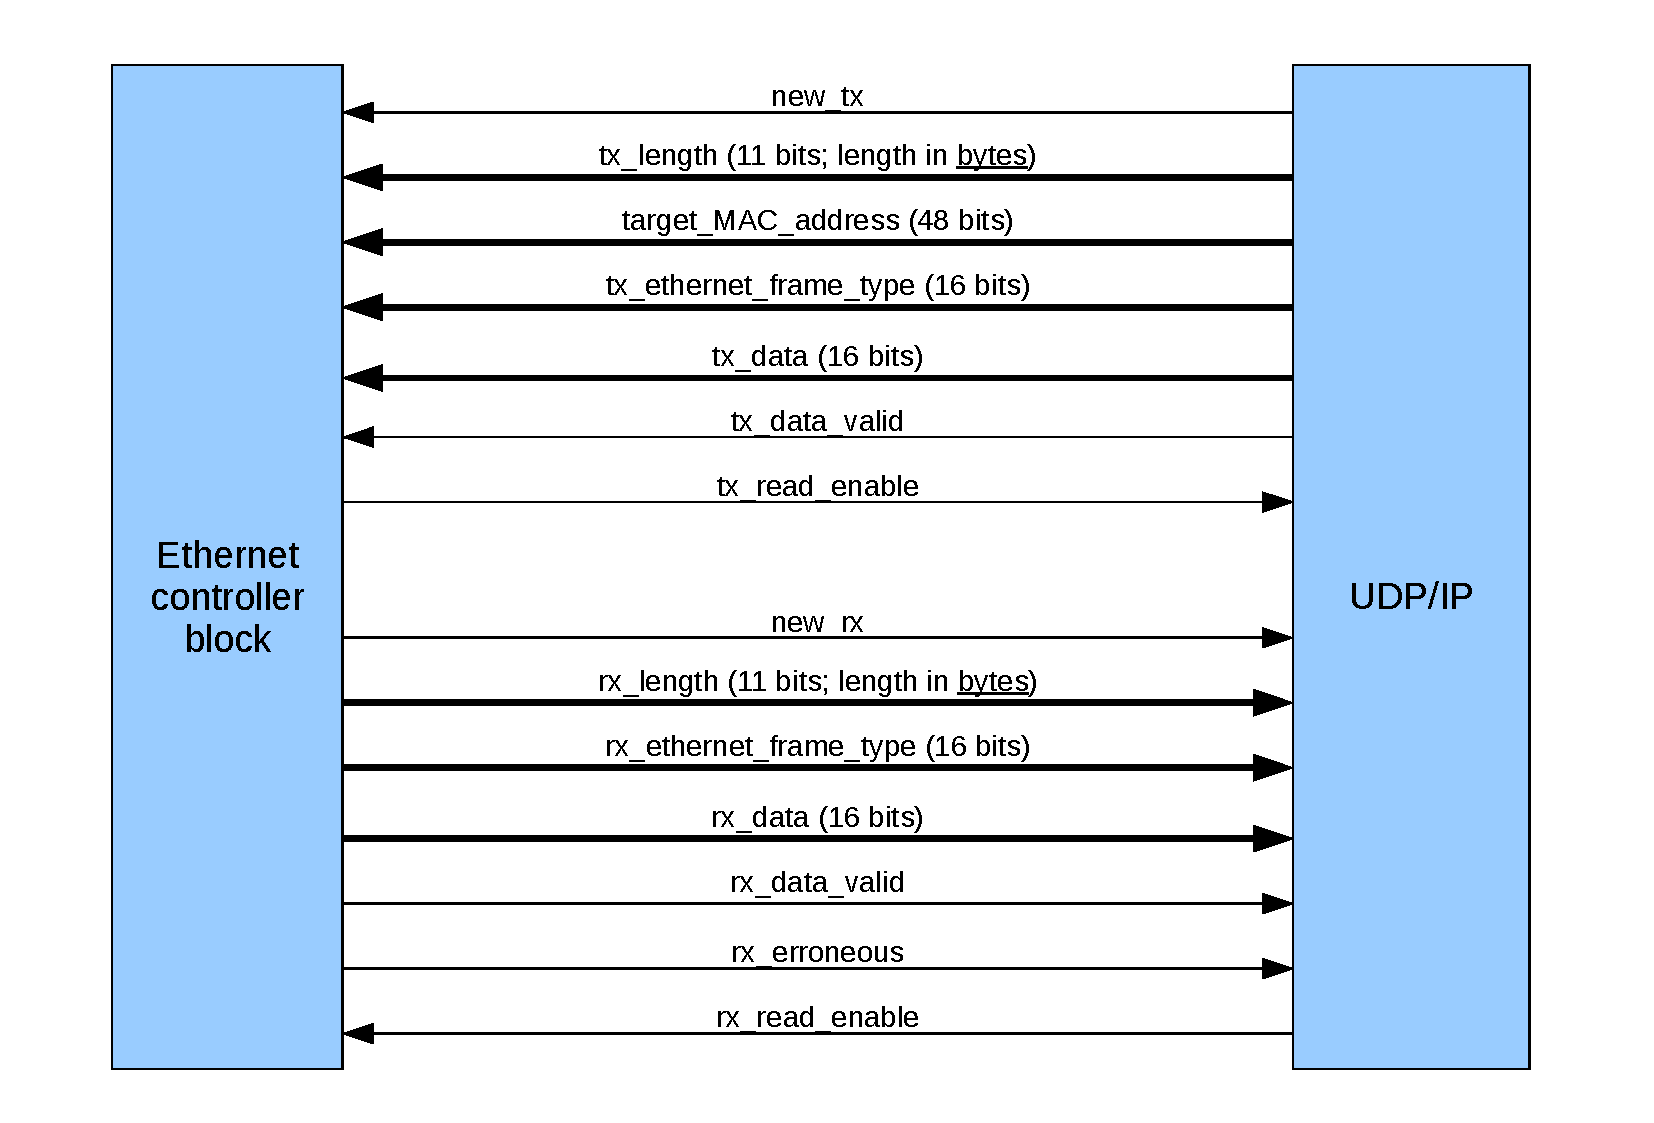
\includegraphics[scale=.5]{fig/eth_interface.pdf}
  \caption{Interface between an ethernet controller block and the UDP/IP block.}
  \label{fig:ethinterface}
\end{figure}


\begin{figure}[hbtp]
  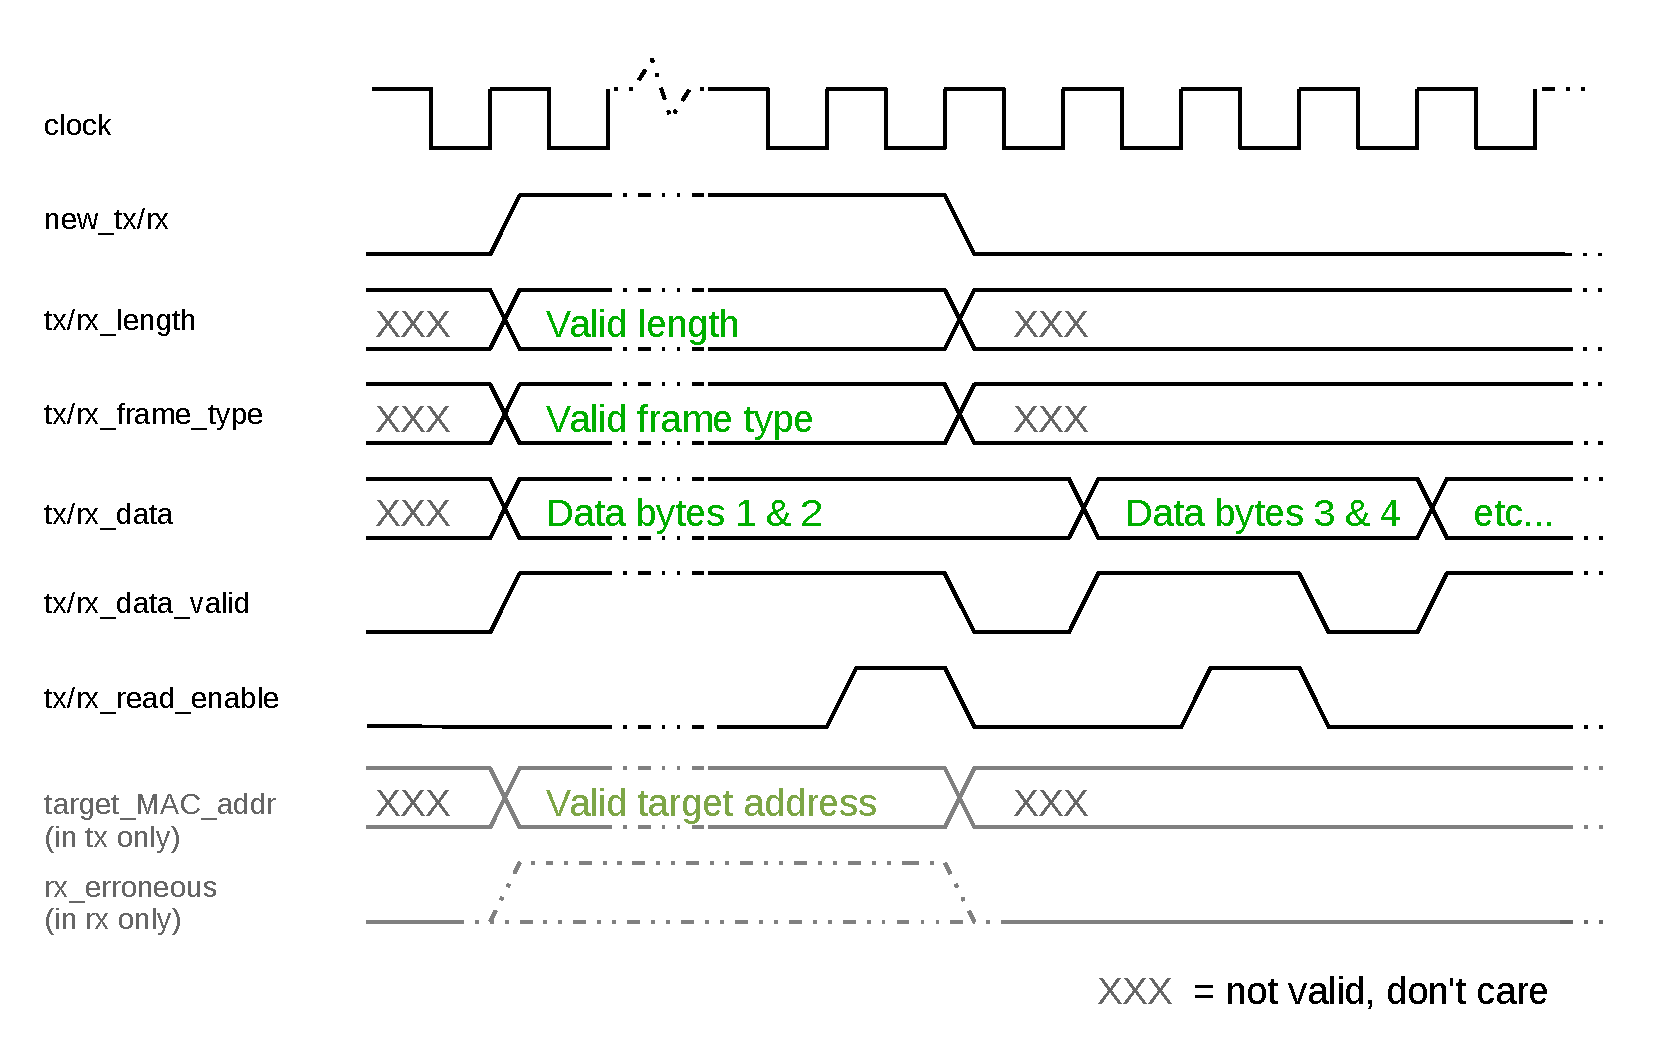
\includegraphics[scale=.5]{fig/eth_timing.pdf}
  \caption{Timing for communication between UDP/IP and ethernet controller block.}
  \label{fig:ethtiming}
\end{figure}


\FloatBarrier
\newpage

\section{IMPLEMENTATION DETAILS} \label{sec:implementation}

This section briefly describes how the UDP/IP block is implemented.
If you aren't making any changes to the source code you hopefully
don't have to care about the following stuff.


\subsection{Structure of the UDP/IP block}

\begin{figure}[hbtp]
  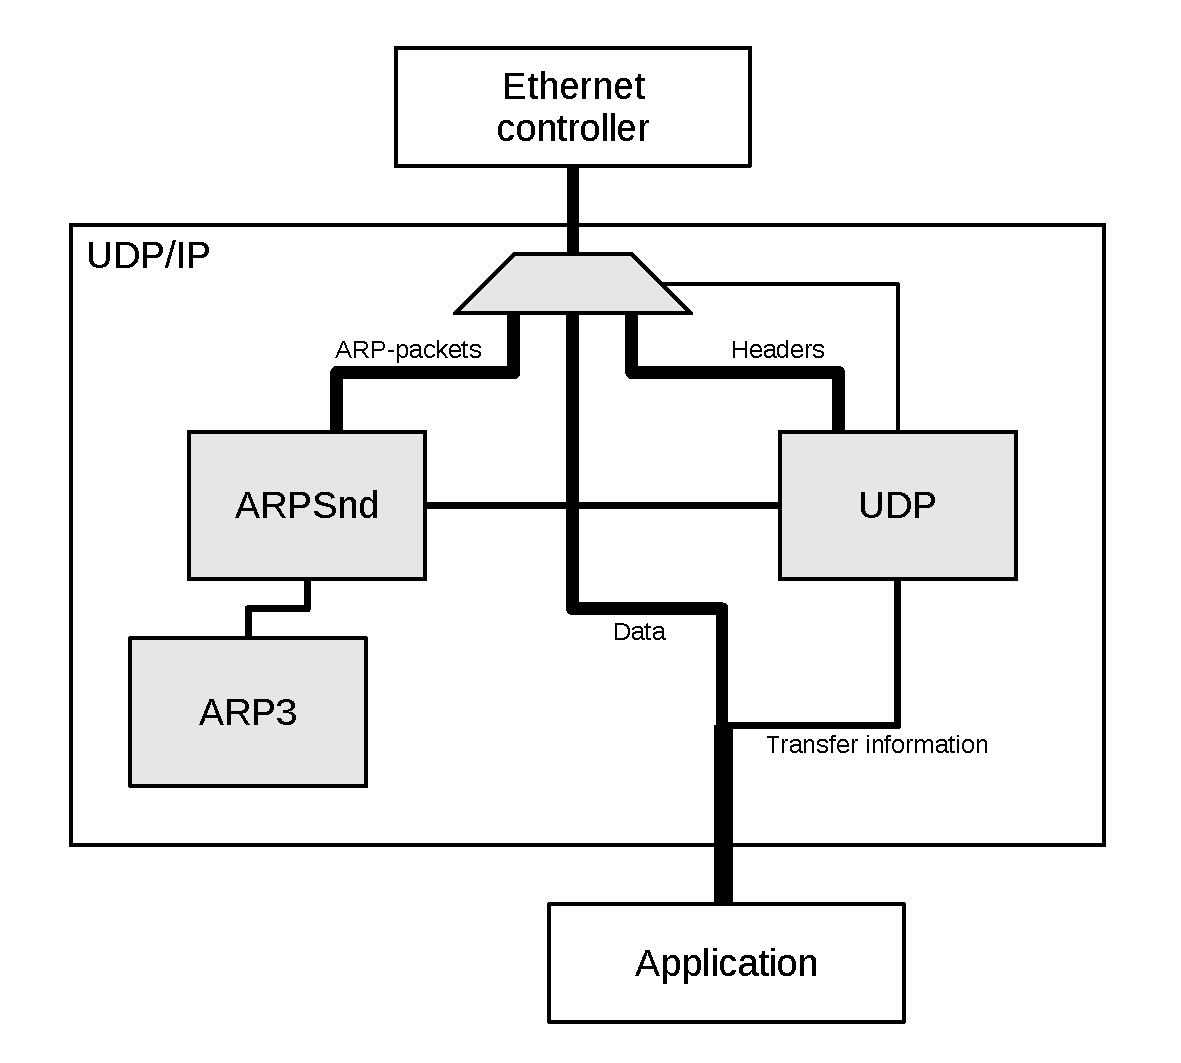
\includegraphics[scale=.6]{fig/system_overview.pdf}
  \caption{Block diagram of the system.}
  \label{fig:system}
\end{figure}

Figure~\ref{fig:system} shows the construction blocks of the system.
Block named UDP is responsible of running the show: it commands the
ARP side and selects the multiplexer input. Its other main task is to
form or interpret the UDP/IP headers depending on the direction of the
transfer.

The ARP functionality~\cite{arp} is divided into two blocks. The ARP3
(the ''3'' comes from the file name, don't know what it stands for)
block includes the ARP table and is responsible of updating it. The
ARPSnd block is responsible of sending and receiving ARP queries and
it also communicates with the UDP block.

The (de)multiplexer selects one of the three sources/destinations for
data going/coming to/from the ethernet controller. UDP sends and
receives headers and ARPSnd ARP packets. The third data bus goes
directly to the application. So e.g. during an outgoing transfer,
after the UDP block has finished sending headers it switches the mux
to relay data from the application straight into the ethernet
controller.


\subsection{State machines of the UDP block}

The UDP block contains most of the control logics, and it uses two
main and two sub state machines. Main state machines \emph{Tx state}
and \emph{Rx state} are shown in figure~\ref{fig:main_states} and the
sub state machines helping in reading or writing headers are shown in
figure~\ref{fig:sub_states}. The header state machines are used when
the main state machines are in states write/read\_IP/UDP\_headers.

\begin{figure}[!hbtp]
  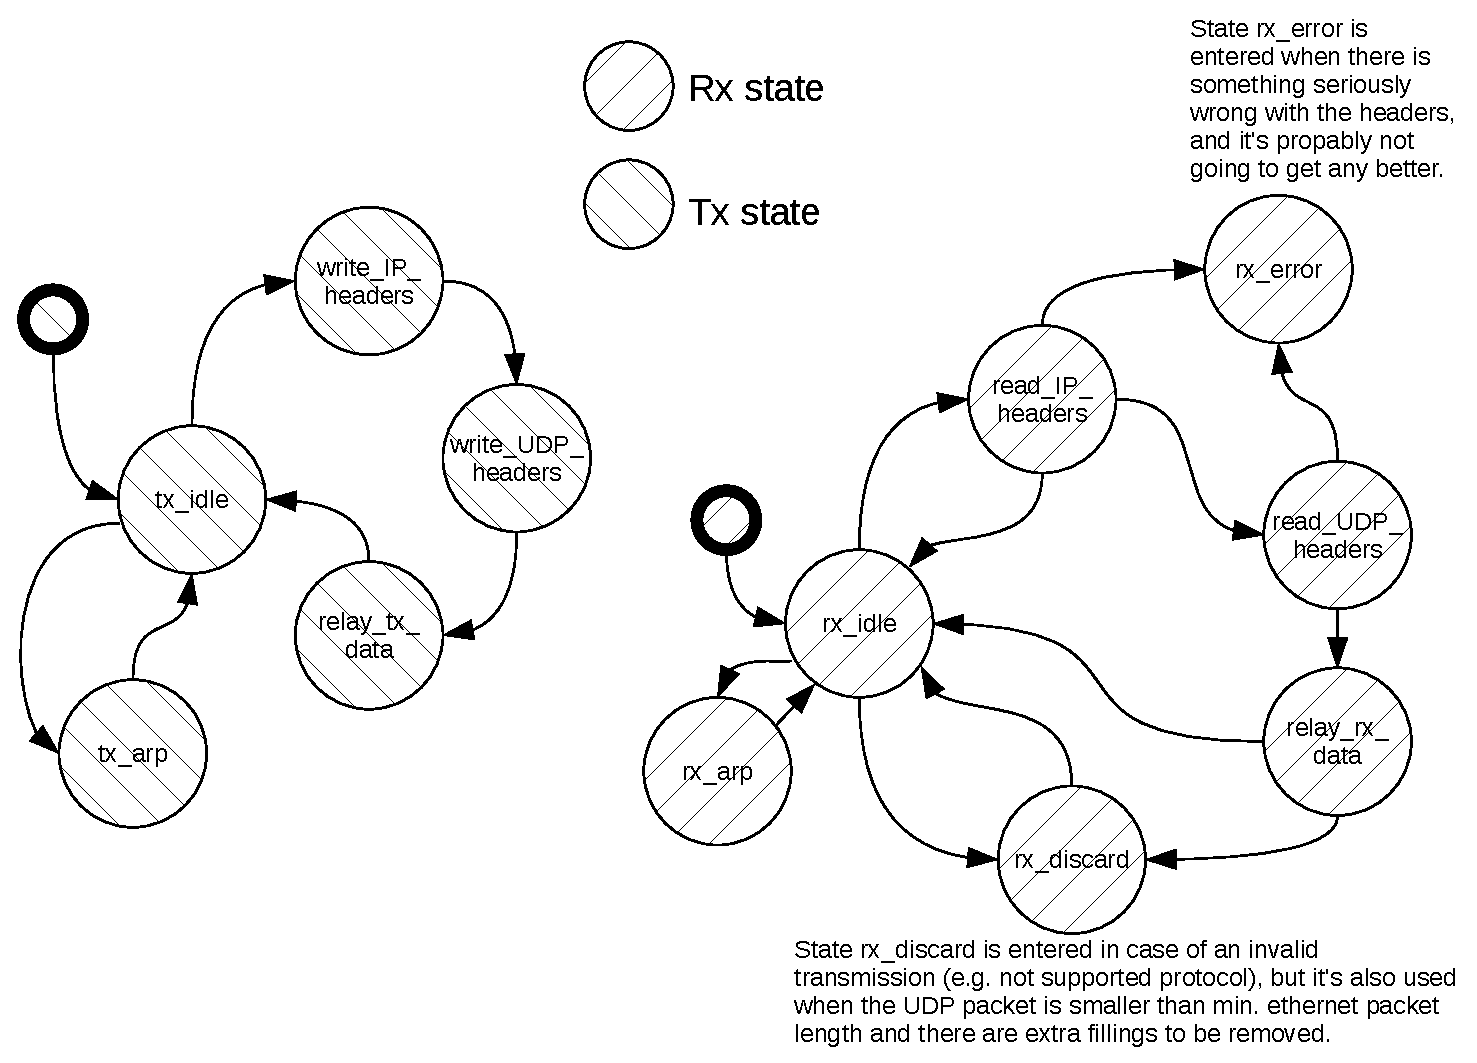
\includegraphics[scale=.5]{fig/udp_block_states.pdf}
  \caption{State diagrams of the two main states.}
  \label{fig:main_states}
\end{figure}

\begin{figure}[!hbtp]
  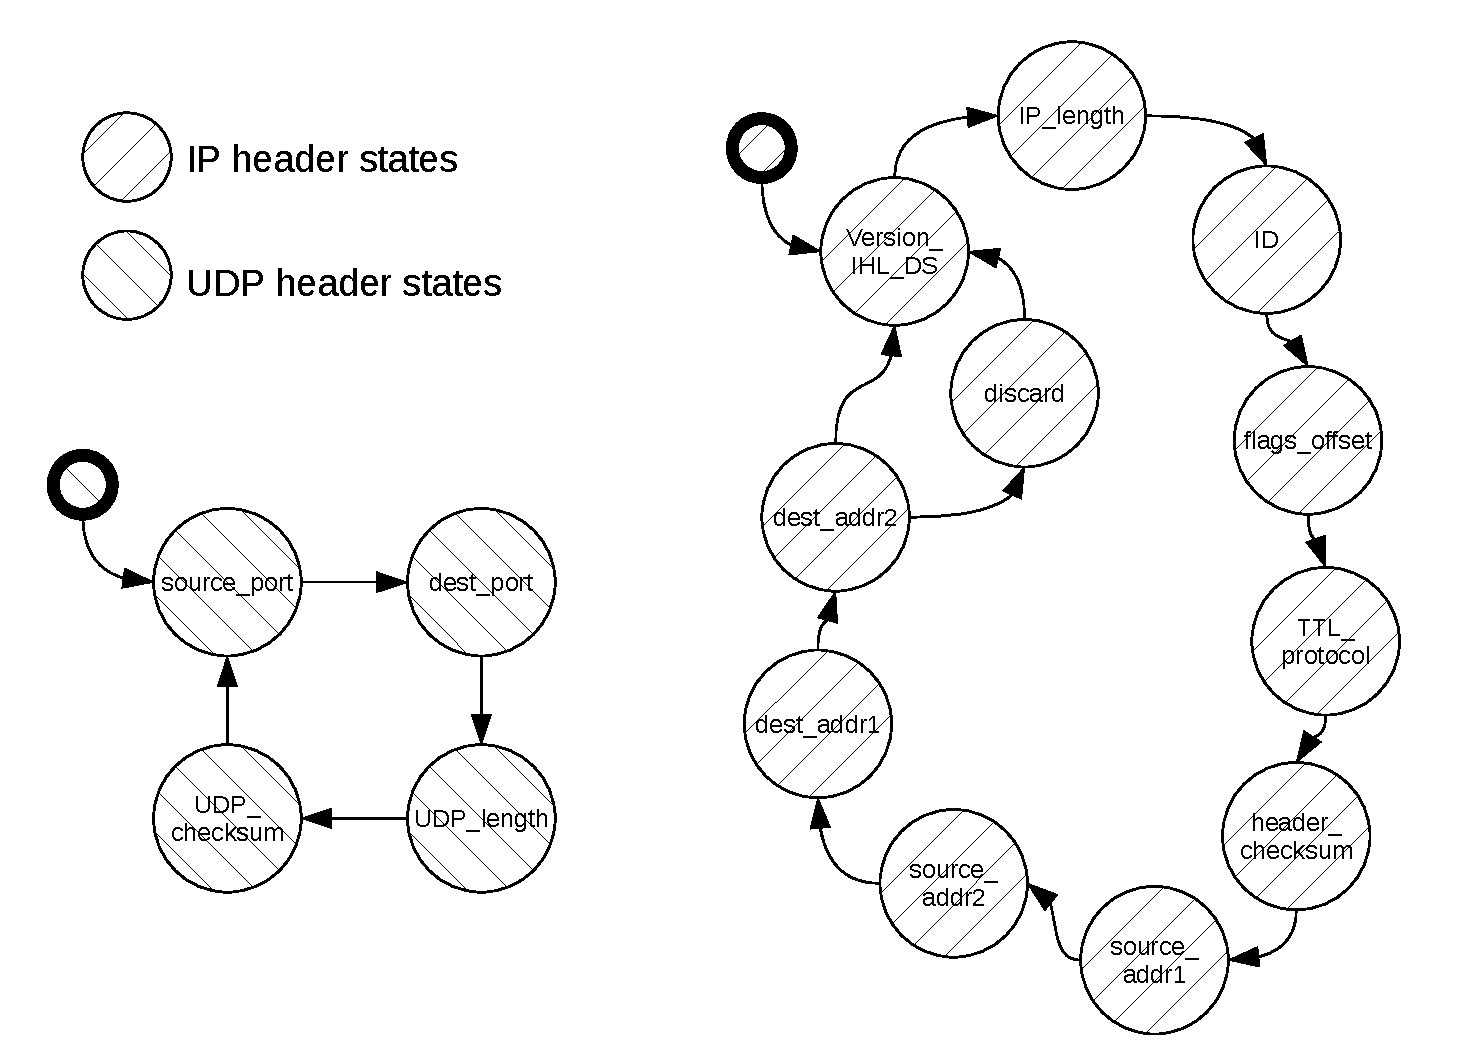
\includegraphics[scale=.5]{fig/header_states.pdf}
  \caption{State diagrams of the header manipulation states.}
  \label{fig:sub_states}
\end{figure}

\subsection{Sending and receiving}

Figures~\ref{fig:sending} and~\ref{fig:receiving} illustrate how
sending and receiving data really happens. I'm not an expert on UML,
so don't mind any unintended semantics. These diagrams are only
trying to show the order in which events take place.

\begin{figure}[!hbtp]
  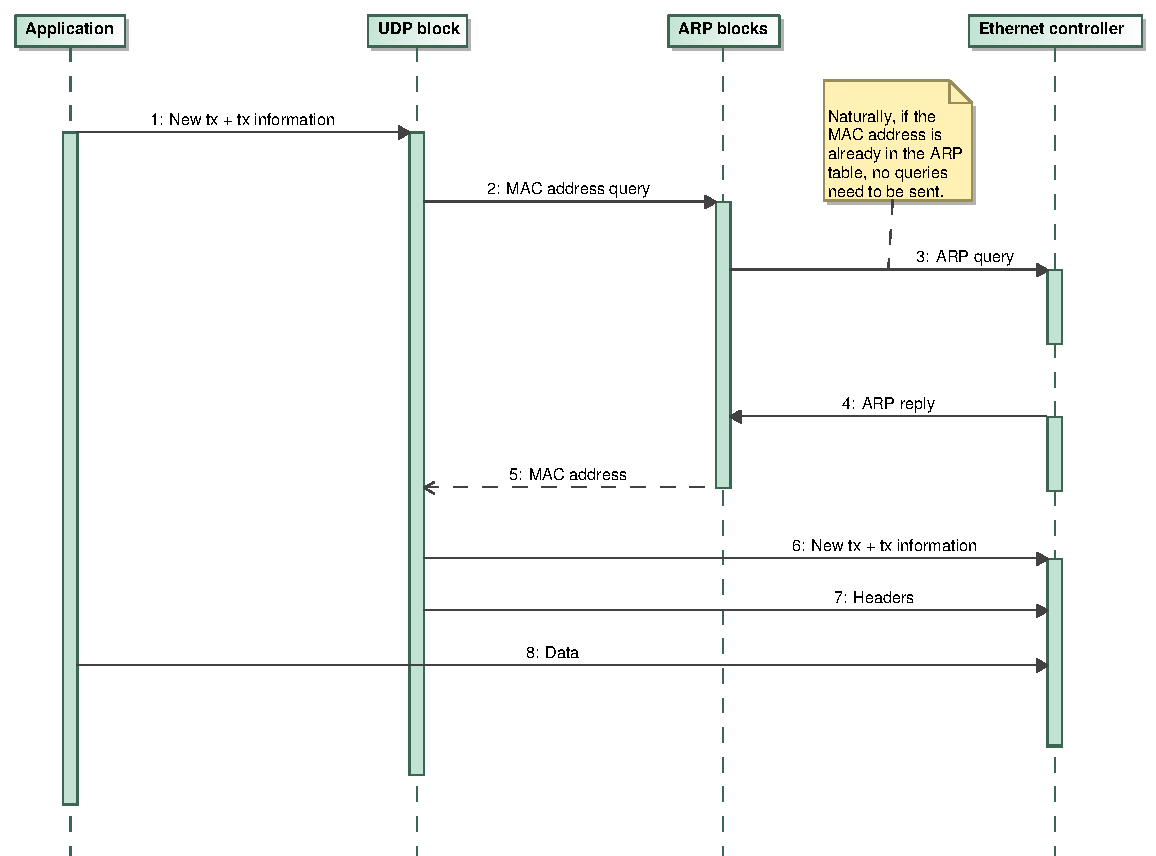
\includegraphics[scale=.65]{fig/sending.pdf}
  \caption{Sequence diagram about sending a packet via UDP/IP.}
  \label{fig:sending}
\end{figure}

\begin{figure}[!hbtp]
  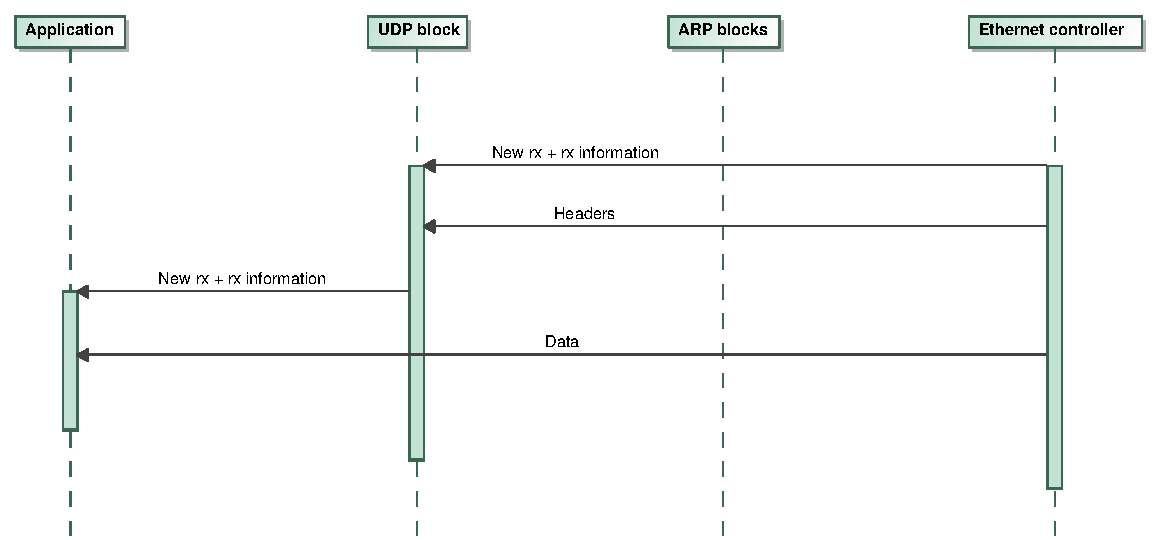
\includegraphics[scale=.65]{fig/receiving.pdf}
  \caption{Sequence diagram about receiving a packet via UDP/IP.}
  \label{fig:receiving}
\end{figure}


\FloatBarrier
\newpage

\addcontentsline{toc}{section}{References} % Lis�� t�m�kin sis�llysluetteloon
\begin{thebibliography}{99}
\bibitem{arp} Ashley Partis, Jorgen Peddersen. VHDL IP Stack Project.
  University of Queensland, Australia, 2001.
  URL:~http://www.itee.uq.edu.au/$\sim$peters/xsvboard/index.html
\end{thebibliography}

  

\end{document}
